% Sample Dissertation, Thesis, or Document %
%            for use with the              %
%  University of Arizona Thesis Class,     %
%               uathesis.cls               %
%------------------------------------------%

% We'll use the uathesis document class (duh).  The uncommented line
% below will produce a Dissertation, the others would produce a Thesis
% or a Document.  There are other options available to you like turning
% on the copyright statement and replacing the year on the title page
% with a "generated on" stamp (handy for early drafts).  To find out
% what the available options are, take a look into the uathesis.cls
% file and look for the \DeclareOption commands near the top of that
% file.
% There are five copyright options.  Copyright, no copyright, and three
% different Creative Commons licences.  Use the one you want (If you go
% Creative Commons, I (DM) think the CC-BY-ND makes the most sense)  See
% uathesis.cls for the reason why the non-commercial licenses are not
% included.
\documentclass[dissertation,openright,oneside]{uathesis}
%\documentclass[dissertation,copyright]{uathesis}
%\documentclass[dissertation,CC-BY]{uathesis}
%\documentclass[dissertation,CC-BY-SA]{uathesis}
%\documentclass[dissertation,CC-BY-ND]{uathesis}
%\documentclass[thesis]{uathesis}
%\documentclass[document]{uathesis}

% Package Usage
% These are the packages that we need
\usepackage{graphicx}
\usepackage[square,numbers]{natbib}
\usepackage[titles]{tocloft}
\usepackage{amsmath}
\usepackage{amssymb}
\usepackage{epstopdf}
\usepackage{dcolumn}% Align table columns on decimal point
\usepackage{bm}% bold math
\usepackage{setspace}
\usepackage{rotating}
\usepackage{csvsimple}
\usepackage[caption=false,font=footnotesize]{subfig}
\usepackage{fixltx2e}
\usepackage[section]{placeins}
\usepackage{textcomp}
\usepackage{tabularx}
\usepackage{booktabs}


\renewcommand*\cftfigpresnum{Figure~}
\setlength{\cftfignumwidth}{5.5em}
\renewcommand\cftchapfont{\normalfont}
\renewcommand\cftchappagefont{\normalfont}
\renewcommand\cftchapleader{\cftdotfill{\cftsecdotsep}}

\newcommand*{\etal}{\emph{et al.}~}

% of the American Astronomical Society.
%\usepackage{deluxetable}		% Allows use of AASTEX deluxe tables
%\usepackage{aastex_hack}		% Allows other AASTEX functionality.

% These are other packages that you might find useful.
% For controlling the fonts, see
% http://www.math.uiuc.edu/~hartke/computer/latex/survey/survey.html
% The following is a nice font set:
%\usepackage{mathtime}			% Times for letters; Belleek math.
%
%\usepackage{lscape}			% Used for making fitting large tables in by putting them landscape
%\usepackage{refs}
%
% If you are using hyper-ref (recommended), this command must go after all
% other package inclusions (from the hyperref package documentation).
% The purpose of hyperref is to make the PDF created extensively
% cross-referenced.
\usepackage[pdftex,bookmarks,colorlinks=true,urlcolor=black,linkcolor=black,citecolor=black]{hyperref}
\usepackage[capitalise]{cleveref}


% Set up some values
\completetitle{Short-Term Irradiance Forecasting Using an Irradiance
  Monitoring Network, Satellite Imagery, and Data Assimilation}
\fullname{Antonio Tomas Lorenzo}
\degreename{Doctor of Philosophy}	% Title of your degree.

\begin{document}
\newcommand{\beq}{\begin{eqnarray}}
\newcommand{\eeq}{\end{eqnarray}}
\newcommand{\ii}{{\mathrm i}}

% Set up the title page
\maketitlepage
{COLLEGE OF OPTICAL SCIENCES}
{2017}

% Insert the approval form.  Note that for electronic submission
% of your Ph. D. dissertation, you must bring *two* copies of the
% approval page to your final defense.  These must be signed by
% the committee.  Make two photocopies: one for Pam and the other
% for your records.  Then, bring the two signed originals to the
% graduate college when you submit the final version of the
% dissertation to the University of Arizona.
\approval
{14 April 2017}		% Defense Date
{Alexander D. Cronin}	% Dissertation Director
{Matthias Morzfeld}
{Alexander D. Cronin}	% 1st committee member
{Matthias Morzfeld}
{Barrett G. Potter Jr.}


% Include the ``Statement by Author'' for Dissertations
\statementbyauthor
% If this is a Thesis, use the following form, with your thesis director's
% name and title in the square brackets like so (you should also omit the
% approval form insertion above):
%\statementbyauthor[Jane M. Doe\\Professor of Chemistry]

% Include the ``Acknowledgements''
\incacknowledgements{acknowledgements}

% Include the ``Dedication''
%\incdedication{dedication}

% Create a ``Table of Contents''
\tableofcontents

% Create a ``List of Figures''
\listoffigures

% Create a ``List of Tables''
\listoftables

% Include the ``Abstract''
\incabstract{abstract}

% Include the various chapters
\chapter{INTRODUCTION}
\label{chap:intro}

The installed capacity of solar power in the US continues to grow as a
result of aging coal and natural gas power plants, lower costs,
state renewable portfolio standards, and efforts to decarbonize the
electrical grid.
As shown in \Cref{fig:solarinstall}, this growth has been steady since 2010 and shows no signs of abating.

\begin{figure}[ht]
  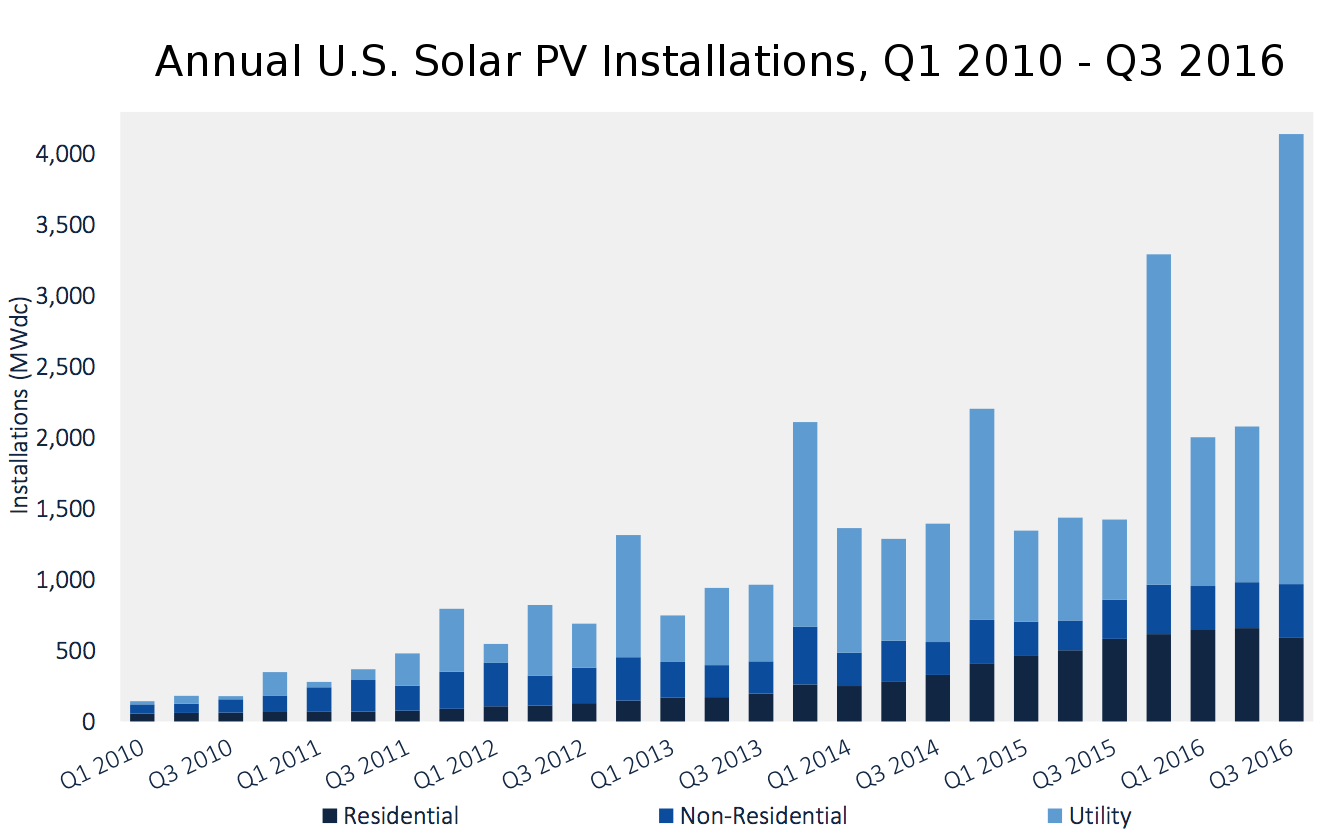
\includegraphics[width=\textwidth]{figs/solar_installations.png}
  \caption[Annual installations of solar PV in the US]{Annual
    installations of solar photovoltaic (PV) systems in the
    US. [Source:~\cite{GTM/SEIA2016}]}
\label{fig:solarinstall}
\end{figure}

Solar irradiance is the fuel that drives all solar power plants.
Unlike sources of fuel for conventional power generators like coal or
natural gas, the solar resource is highly variable due to the nature
of the chaotic system that is weather.
This variability of the solar resource leads to uncertainty at the
electric utility and increases management costs \citep{Joskow2011}.
Forecasts help utilities manage the variability in a number of ways
\citep{Kleissl2013,Inman2013}, including the optimal dispatch of
battery storage \citep{Cormode2015}.

This dissertation will explore solar irradiance forecasting at short
time horizons (now to two hours in the future) made possible by an
irradiance monitoring network.
First, the current state of solar power in the Southwest US and a
brief overview of forecasting methods will be discussed.

\section{State of Solar Power in the Southwest}
duck curve

a bit of SVERI analysis

how much solar total?
percentage of load?

nice heatmap

DG and visibility of DG


\section{Solar Irradiance Forecasting}
nowcasting DG

other techniques

little bit about WRF

\begin{figure}[h]
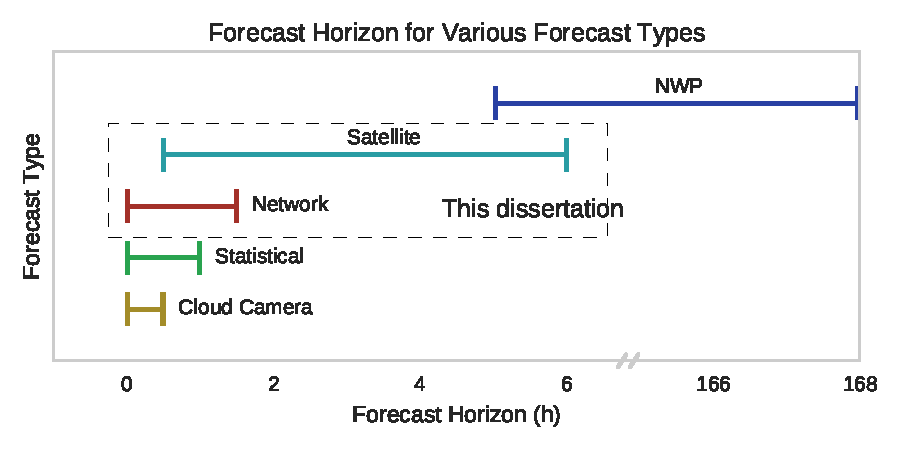
\includegraphics[width=\textwidth]{figs/fxhoriz.pdf}
\caption[Forecast horizon for various forecast types]{The optimal
  forecast horizons for various types of short-term forecasts. This
  dissertation will focus on network and satellite forecasts.}
\label{fig:fxhoriz}
\end{figure}


\section{This Dissertation in Brief}

\begin{figure}[h]
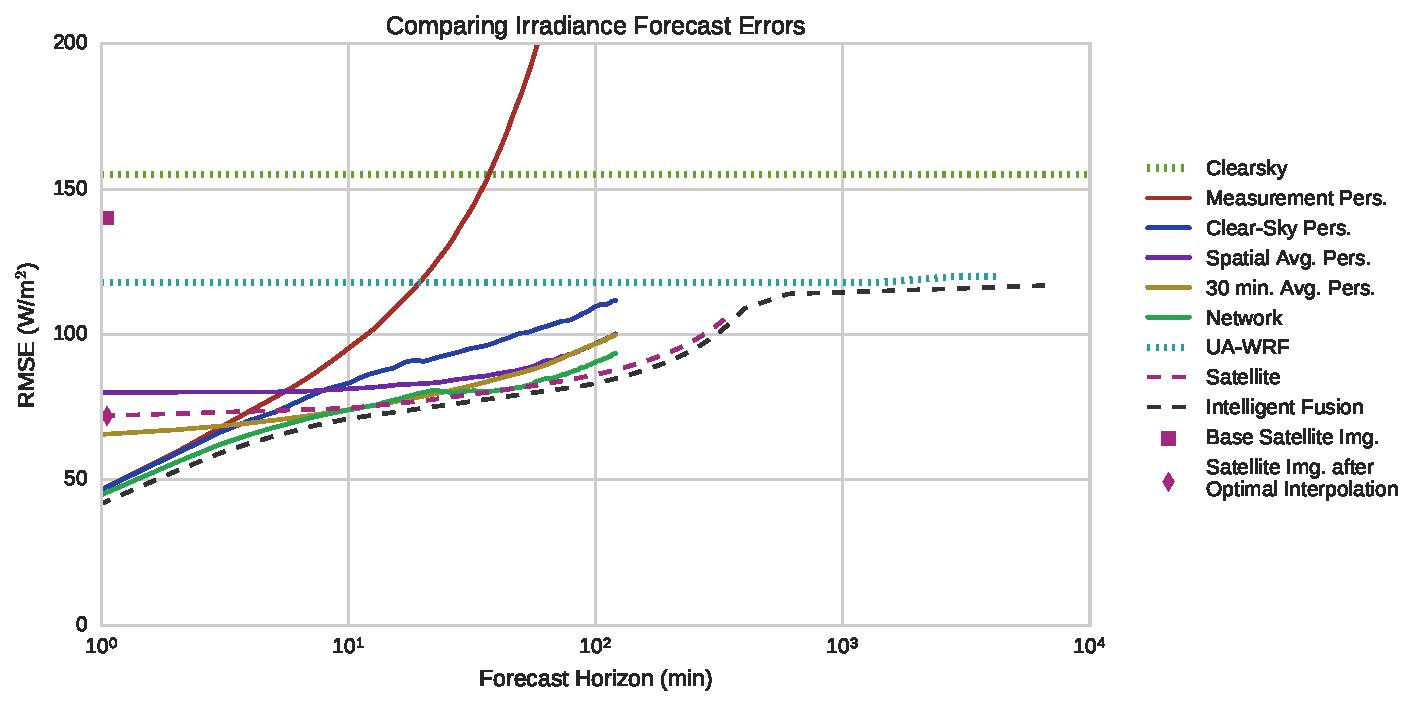
\includegraphics[width=\textwidth]{figs/timehorizon.pdf}
\caption[Irradiance forecast errors across forecast horizons]{A
  comparison of irradiance forecast root-mean squared errors (RMSE)
  across many time horizons. The solid lines (and points) indicate
  forecasts that will be studied in depth in this dissertation. Dashed
  lines are based on prelimnary analysis, but have not been studied in
  depth. Pers.\ refers to persistence, and UA-WRF refers to the
  numerical weather models generated at the UA using the Weather
  Research and Forecasting (WRF) model. The optimal grinding is a
  theoretical combination of forecasts at diffferent time horizons for
  the best forecast at all horizons. The persistence and network
  forecasts will be discussed in \Cref{chap:network} and the satellite
  image points will be discussed in \Cref{chap:satoi}.}
\label{fig:bullshitplot}
\end{figure}




%%% Local Variables:
%%% mode: latex
%%% TeX-master: "dissertation"
%%% End:

\chapter{IRRADIANCE MONITORING NETWORK}
\label{chap:sens_net}

This chapter describes the irradiance monitoring network that was
deployed in Tucson, AZ, and is the basis for much of the forecasting
work in this dissertation.
First, we present some background on why we built the network.
Next, we describe the design of the custom sensors that we deployed as
part of the network.
Then, we discuss how rooftop PV systems can be used as proxies for
irradiance sensors.
Finally, we present possible improvements one might consider for
future networks.

\section{Background}

The initial application of an irradiance monitoring network is laid
out in \cite{Lonij2013}.
Using historical data from 80 residential rooftop PV systems, Lonij
\etal produced intra-hour solar power forecasts that showed skill over
persistence forecasts.
The local electric utility, Tucson Electric Power (TEP), was interested in
receiving these short-term forecasts in real-time.
To generate real-time forecasts, data from sensors need to be gathered
in real-time, thus we set out building the irradiance monitoring
network that would report values in near real-time.

\section{Design of Custom Sensors}
\label{sec:custom_sensors}
This section describes the custom irradiance sensors that were
developed to support the forecasting work in this dissertation.
These sensors were custom designed based upon the lack of available,
low-cost alternatives.
The sensors as described cost around \$500 in raw materials when they
were built in early 2014.
This low cost allowed us to build and deploy many sensors to collect
more data.
The sensors were also desgined to communicate data back in real-time
so that the network could be used to produce operational forecasts for
TEP.

\subsection{Photodiode Sensor}
\label{sec:photodiode}
A number of photodiodes were studied to determine a suitable,
inexpesive replacement for a pyranometer to measure irradiance.
We tested a clear domed photodiode which we sanded to better diffuse
light, a thin sheet of telfon glued on a photodiode to diffuse light,
and a an unmodified, flat photodiode, among others.
We found that the flat photodiode (Osram BPW34) provided a reasonable
signal level and cosine response, shown in \cref{fig:pdshape}.
This photodiode is sufficient to detech changes in the irradiance from
a clear-sky, as a pyranometer would, which is the main way the network
will be used.

\begin{figure}[h]
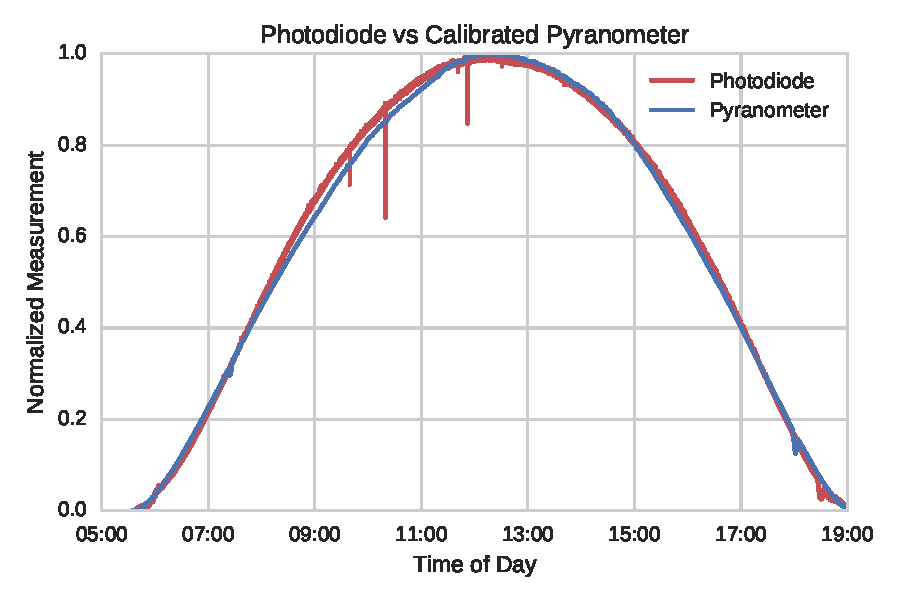
\includegraphics[width=\textwidth]{figs/pdvspy.pdf}
\caption[Comparison of photodiode and pyranometer signals]{A
  comparison of the signal from a photodiode and a calibrated
  pyranometer. The photodiode does not exhibit a perfect cosine
  response with a wider peak that decays too quickly. However, the
  photodiode performs well for the main purpose of detecting changes
  in irradiance. Note that the noise in the measurement of the
  photodiode is about double the noise in the pyranometer measurement.}
\label{fig:pdshape}
\end{figure}

\subsection{Hardware}
\label{sec:senshardware}
A custom printed circuit board was designed for the components that
store and send sensor data to a central server every minute.
The circuit diagram for this board is shown in \cref{fig:circuit}.
Design files for the circuit board can be found online~\cite{sensorrepo}.

\begin{sidewaysfigure}[p]
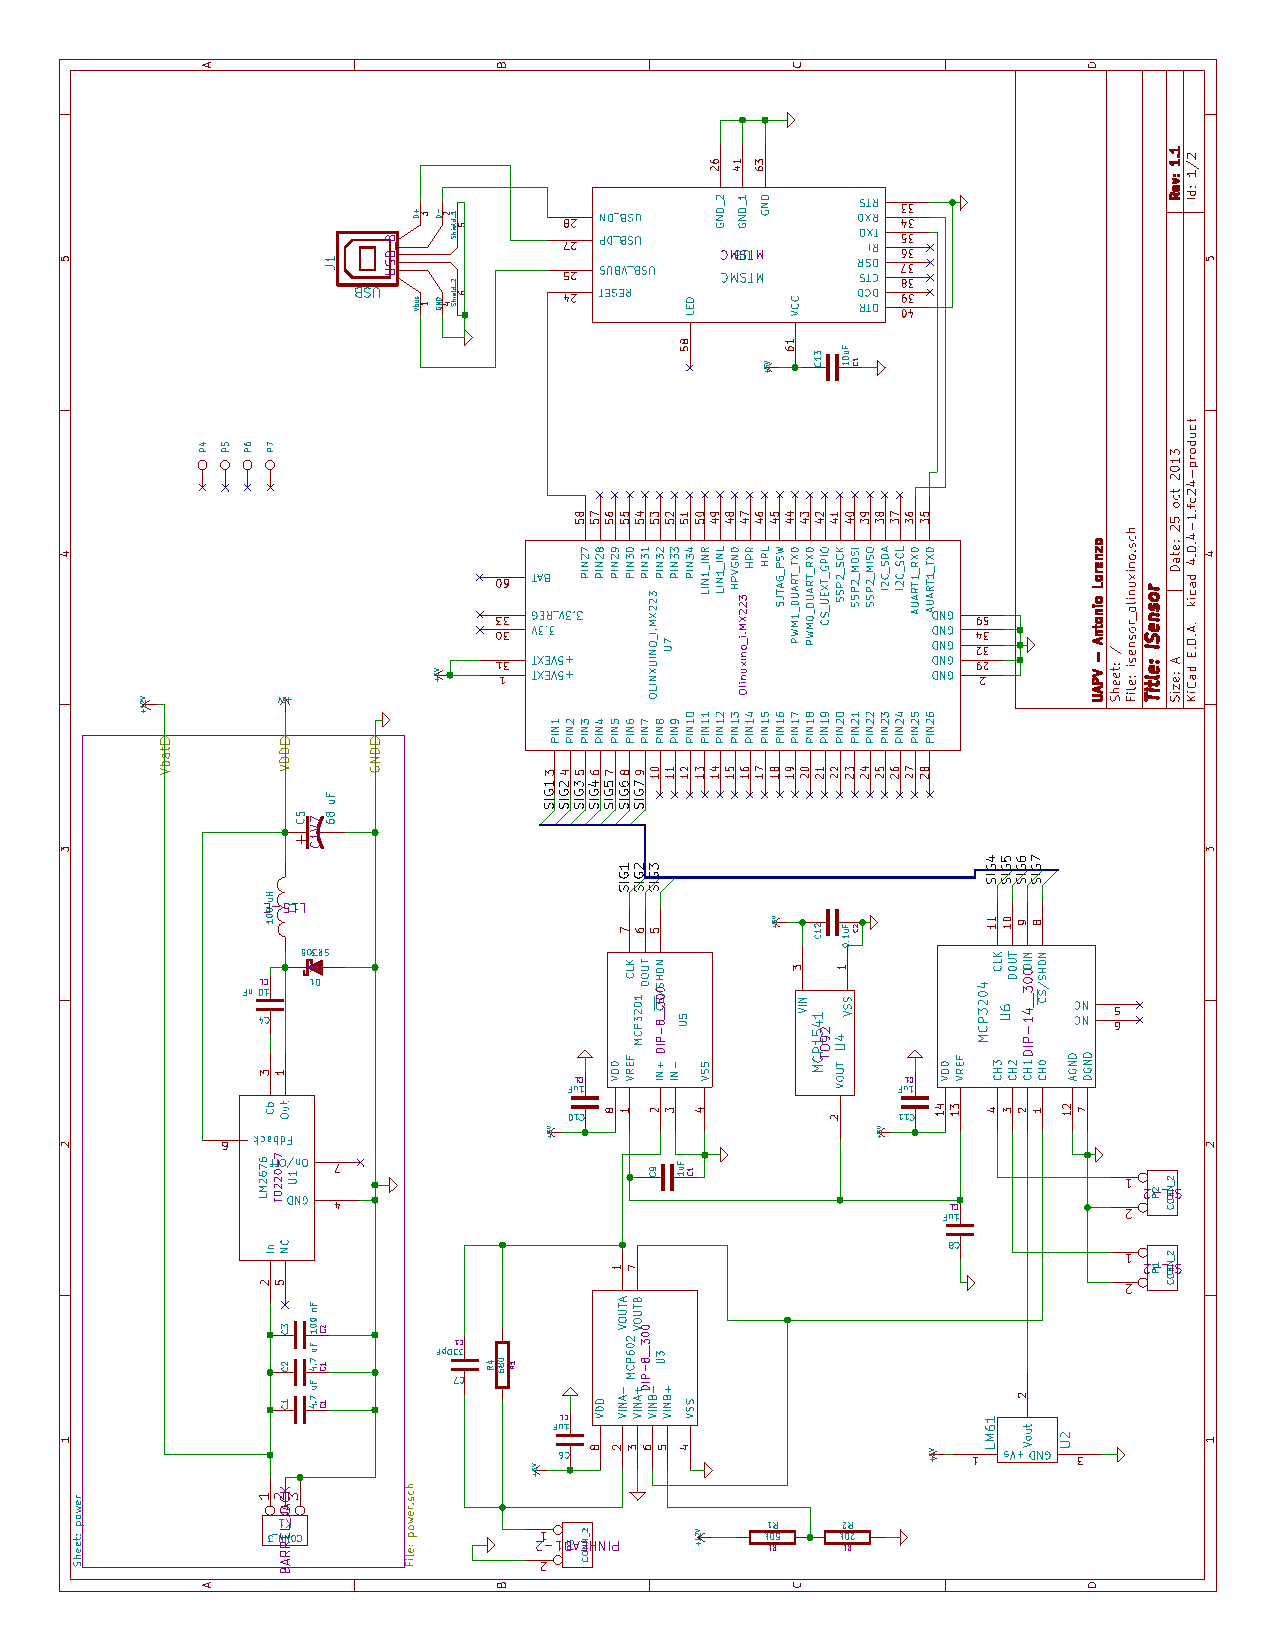
\includegraphics[angle=-90,width=\textwidth]{figs/circuit.pdf}
\caption[Custom sensor circuit diagram]{Circuit diagram for the
  custom, remote irradiance sensors. See \cref{sec:senshardware} for a
  descirpiton of the components.}
\label{fig:circuit}
\end{sidewaysfigure}

The custom sensors are developed around the Olimex
iMX223-OLinuXino-MICRO board.
The OLinuXino was chosen because it consumes little power ($< 1$W) and it
runs a full Linux operating system which allows for development in any
language that can be installed on Linux along with the usual suite of
Linux tools (SSH, Bash, logs).
It is also relatively inexpensive to purchase complete boards, and the
plans are open-source if one desires to build the board themselves.

Data is communicated via GSM using a MULTITECH MTSMC-H5-U SocketModem.
This modem accepts a standard SIM card that is registered with a
cellular data provider.
The modem is connected to the OLinuXino via USB.
WvDial and PPPD are used to setup the connection to the modem and
allow internet access.

Power to the system is provided by a 10W solar panel and a 6Ah
lead-acid battery.
A standard solar charge controller is used limit the current from the
panel to the battery.
The nominal 12V from the battery is routed to the circuit board with
the OLinuXino and modem and converted to 5VDC with a circuit based on
the LM2676 step-down regulator.

The sensor is designed to accept input from either a calibrated
pyranometer (Apogee SP-212) or an inexpensive silicon photodiode
(Osram BPW34) as discussed in \cref{sec:photodiode}.
A trans-impedance amplifier (MCP602) with appropriate gain is used to
convert the current from the photodiode into a measurable voltage.

The voltage from the sensor (or sensor + trans-impedance amplifier) is
converted to a digital signal with the MCP3201 12-bit
analog-to-digital converter (ADC).
This digital signal is then read the OLinuXino at regular intervals
from the GPIO pins.
An additional 4 channel 12-bit ADC (MCP3204) is used to convert other
values such as enclosure temperature (measured by an LM61) and battery
voltage to be read on the OLinuXino GPIO pins for monitoring.
A 4.096V voltage reference (MCP1541) is used by both ADCs.

\begin{figure}[t]
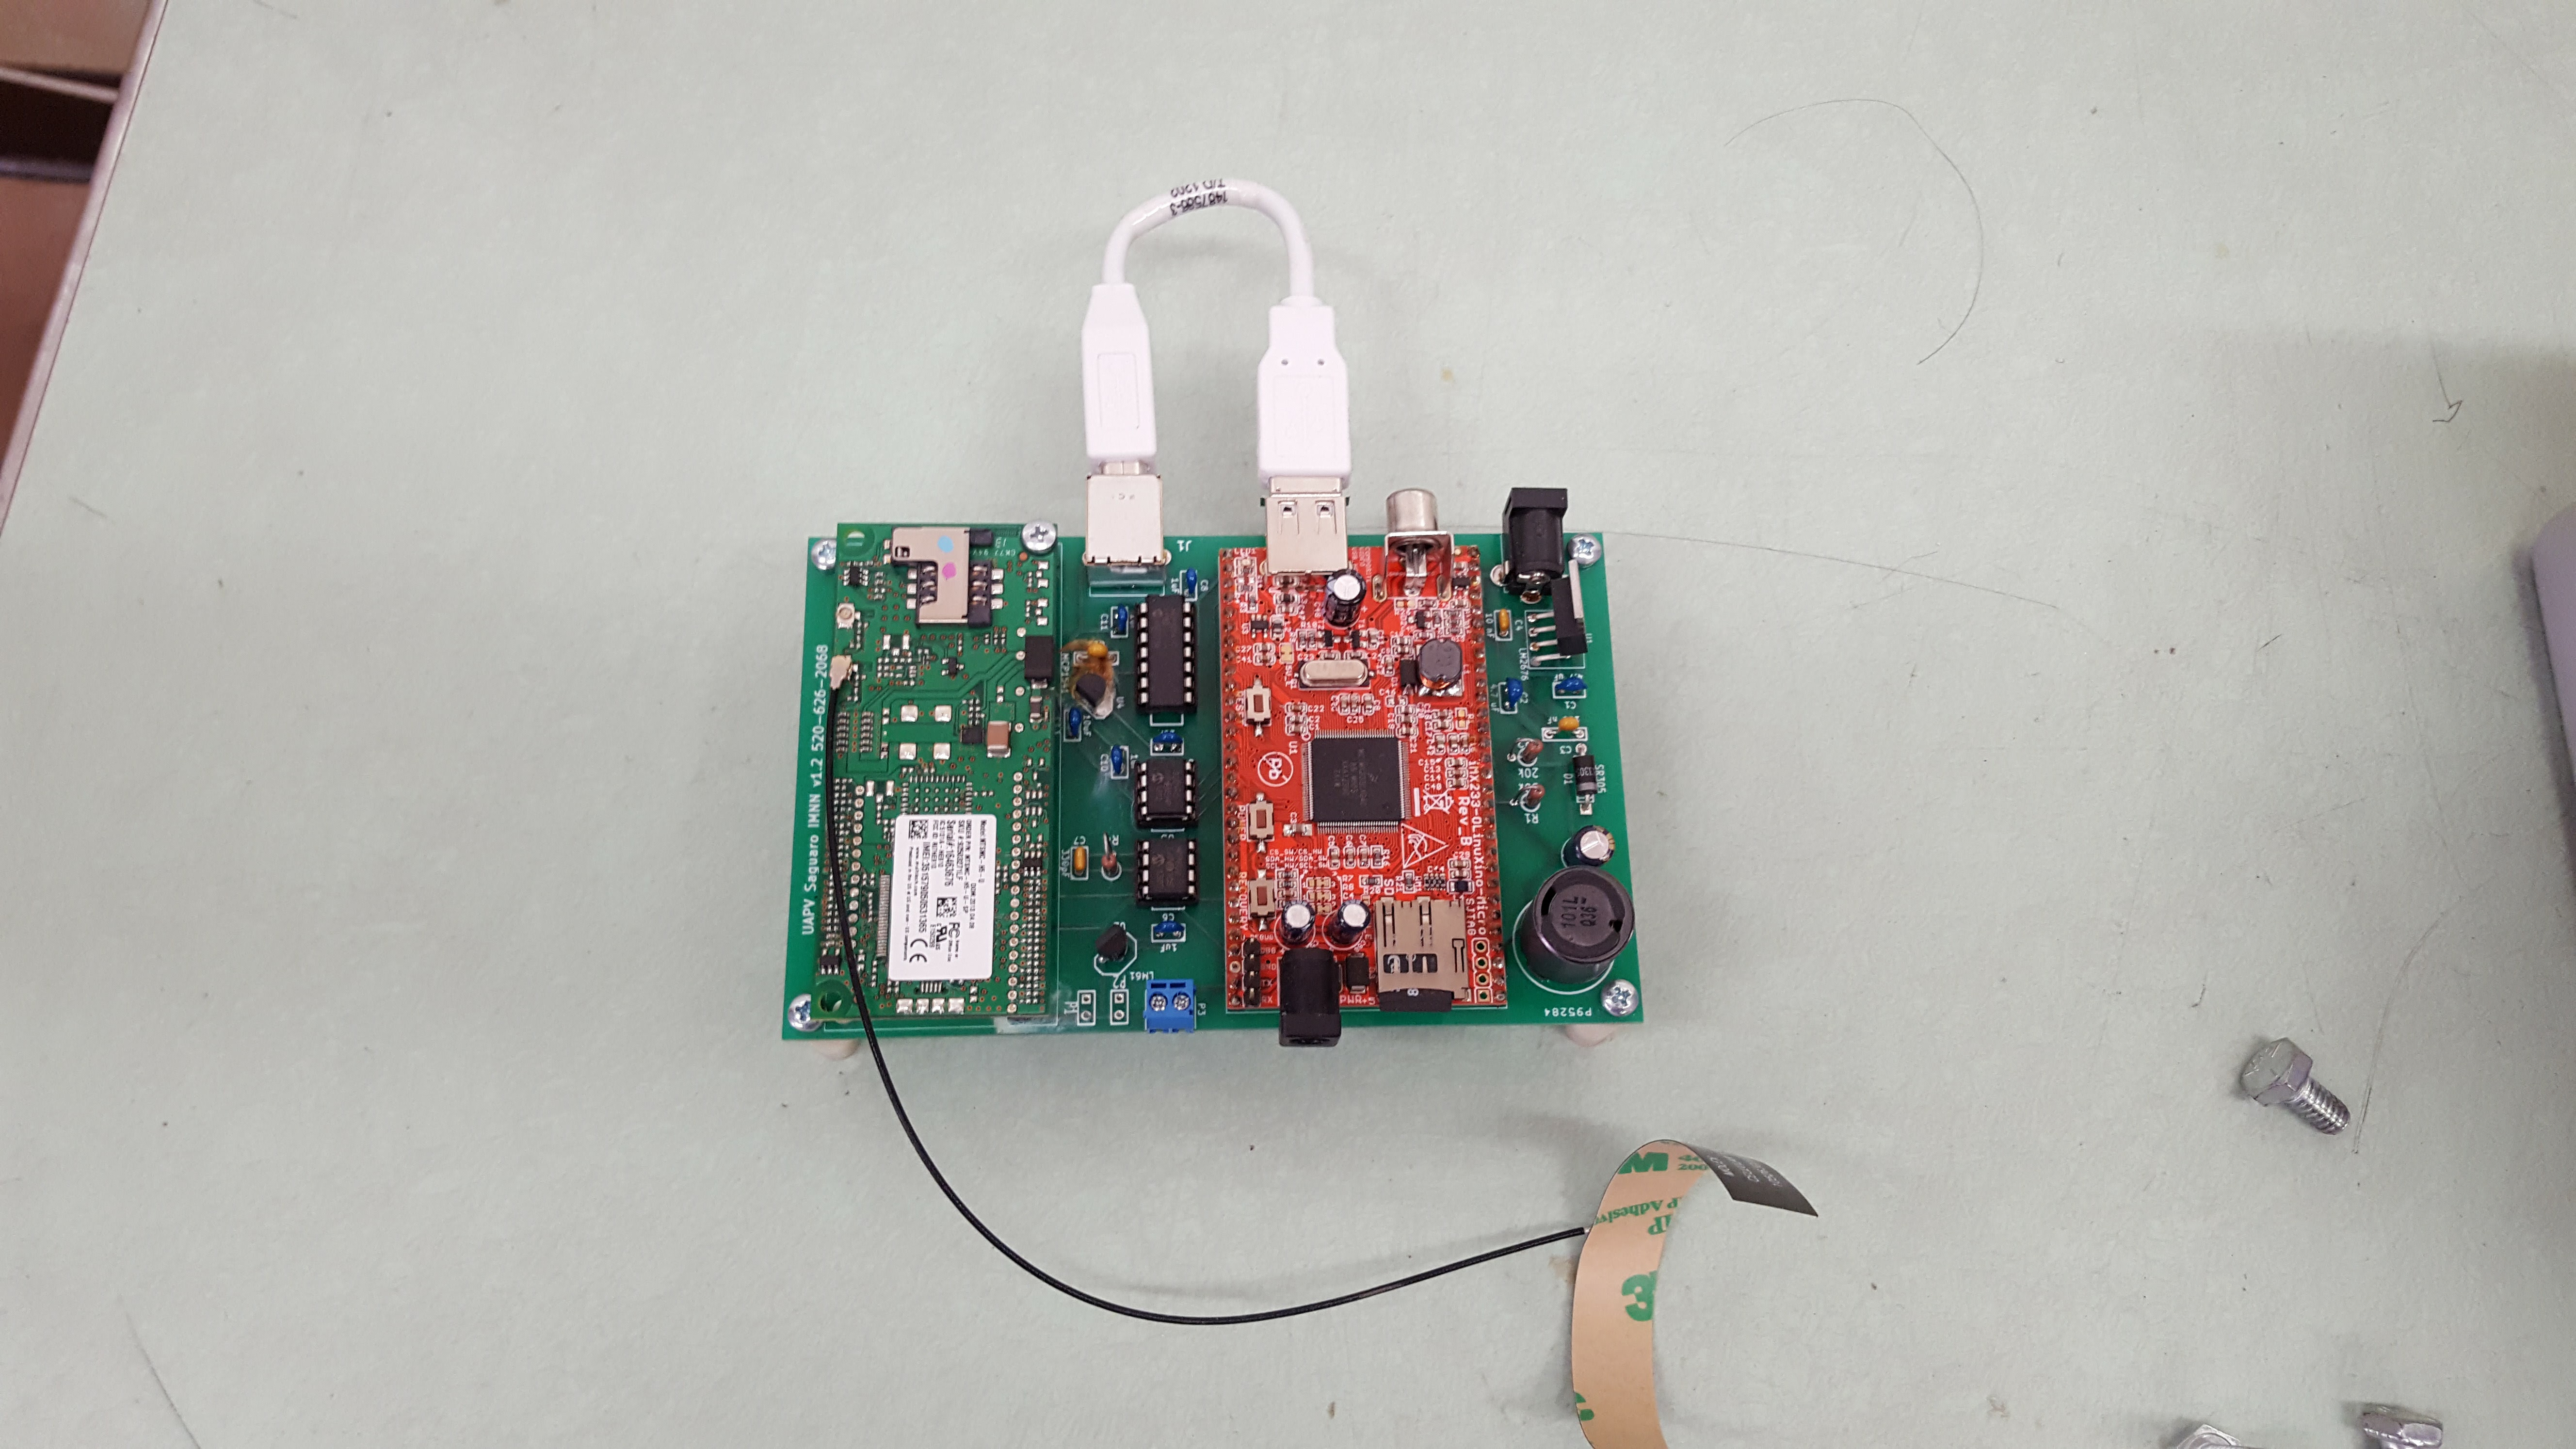
\includegraphics[width=\textwidth]{figs/sensor_board.jpg}
\caption[Assembled sensor circuit board]{A fully assembled printed
  circuit board for a custom sensor. The red board is the OLinuXino
  and the green board on the left is the cell modem with a flexible
  antenna. Through hole components were chosen for easy soldering.}
\label{fig:sensor_board}
\end{figure}

A fully assembled printed circuit board is shown in
\cref{fig:sensor_board}.
The circuit board is housed in a waterproof box with an air snorkel
and cable nipples to maintain water resistance.
A metal extrusion serves as a mast to mount the photodiode or
pyranmeter.
The solar panel and this mast are attached to the top of the
waterproof box which can then be placed outside.
A photo of the interior of the box with the circuit board and lead
acid battery is shown in \cref{fig:sensor_int}.
An entire completed sensor undergoing testing is shown in
\cref{fig:sensor_outside}.

\begin{figure}[ht]
  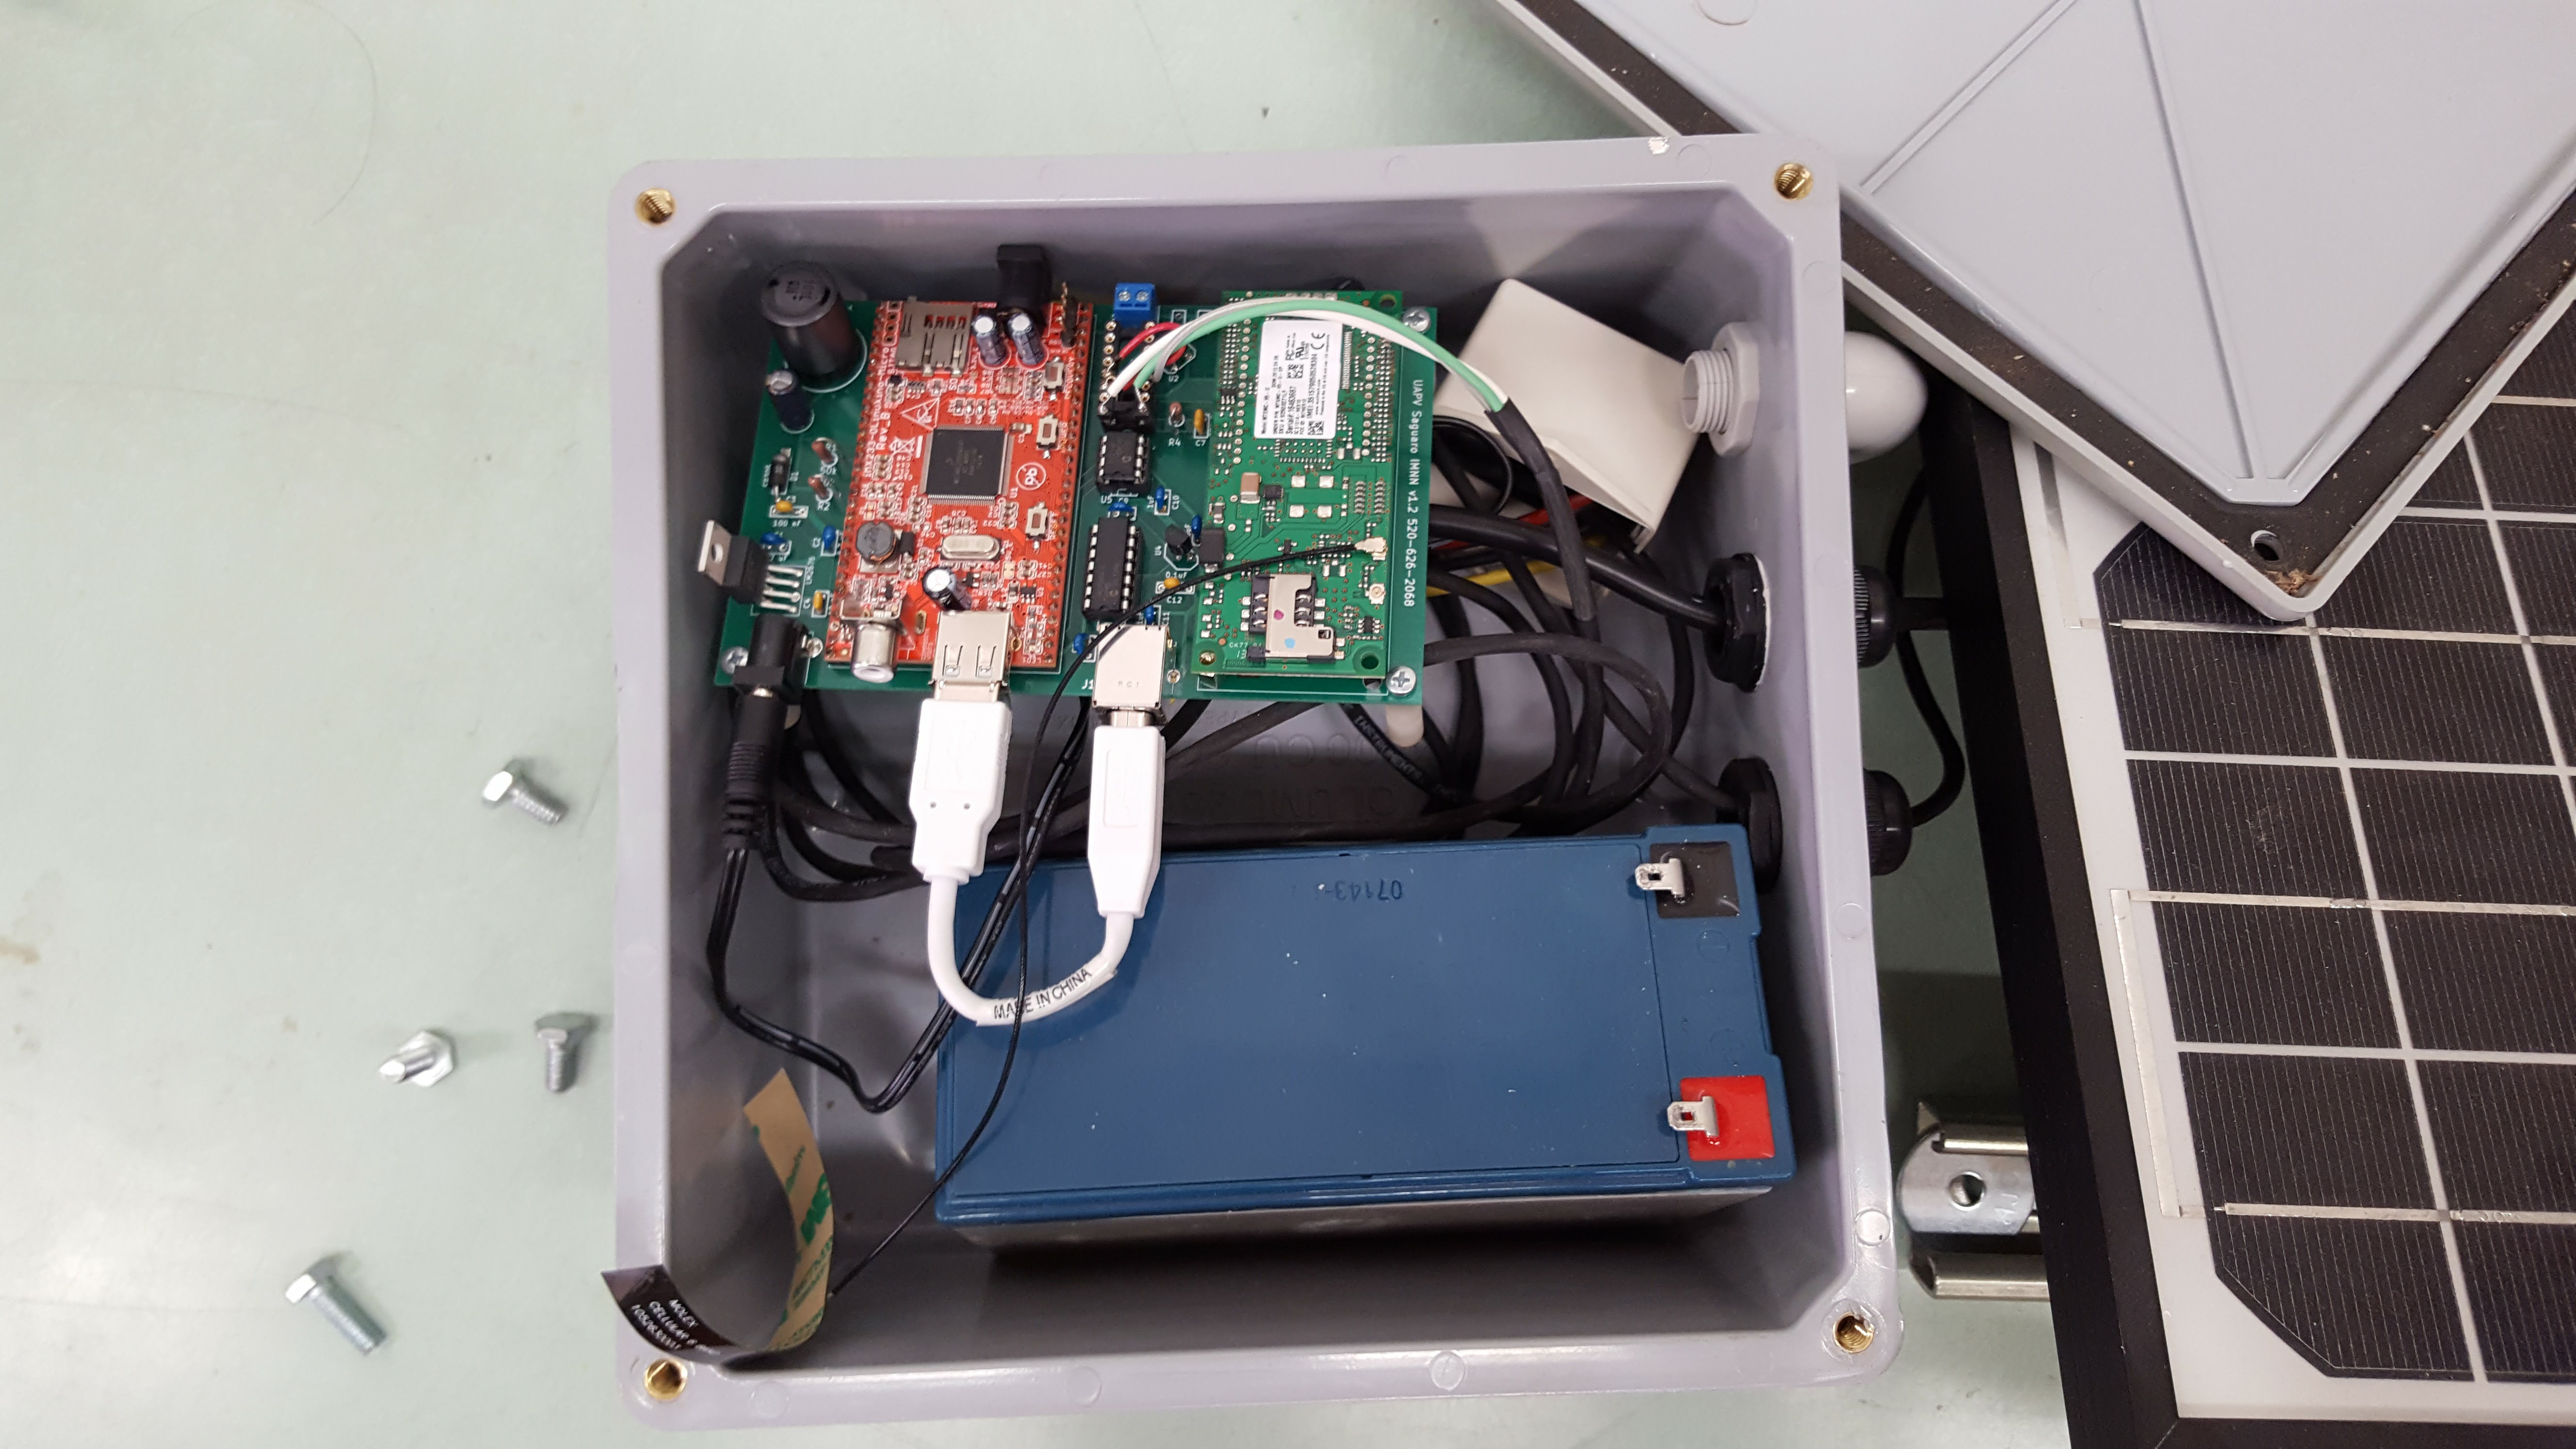
\includegraphics[width=\textwidth]{figs/sensor_interior.jpg}
\caption[Interior of the sensor enclosure]{A photo of the interior of
  the sensor enclosure. The air vent and waterproof cable nipples are
  visible on the right side of the box. The 6Ah 12V motorcycle battery
  is shown near the bottom.}
\label{fig:sensor_int}
\end{figure}

\begin{figure}[p]
  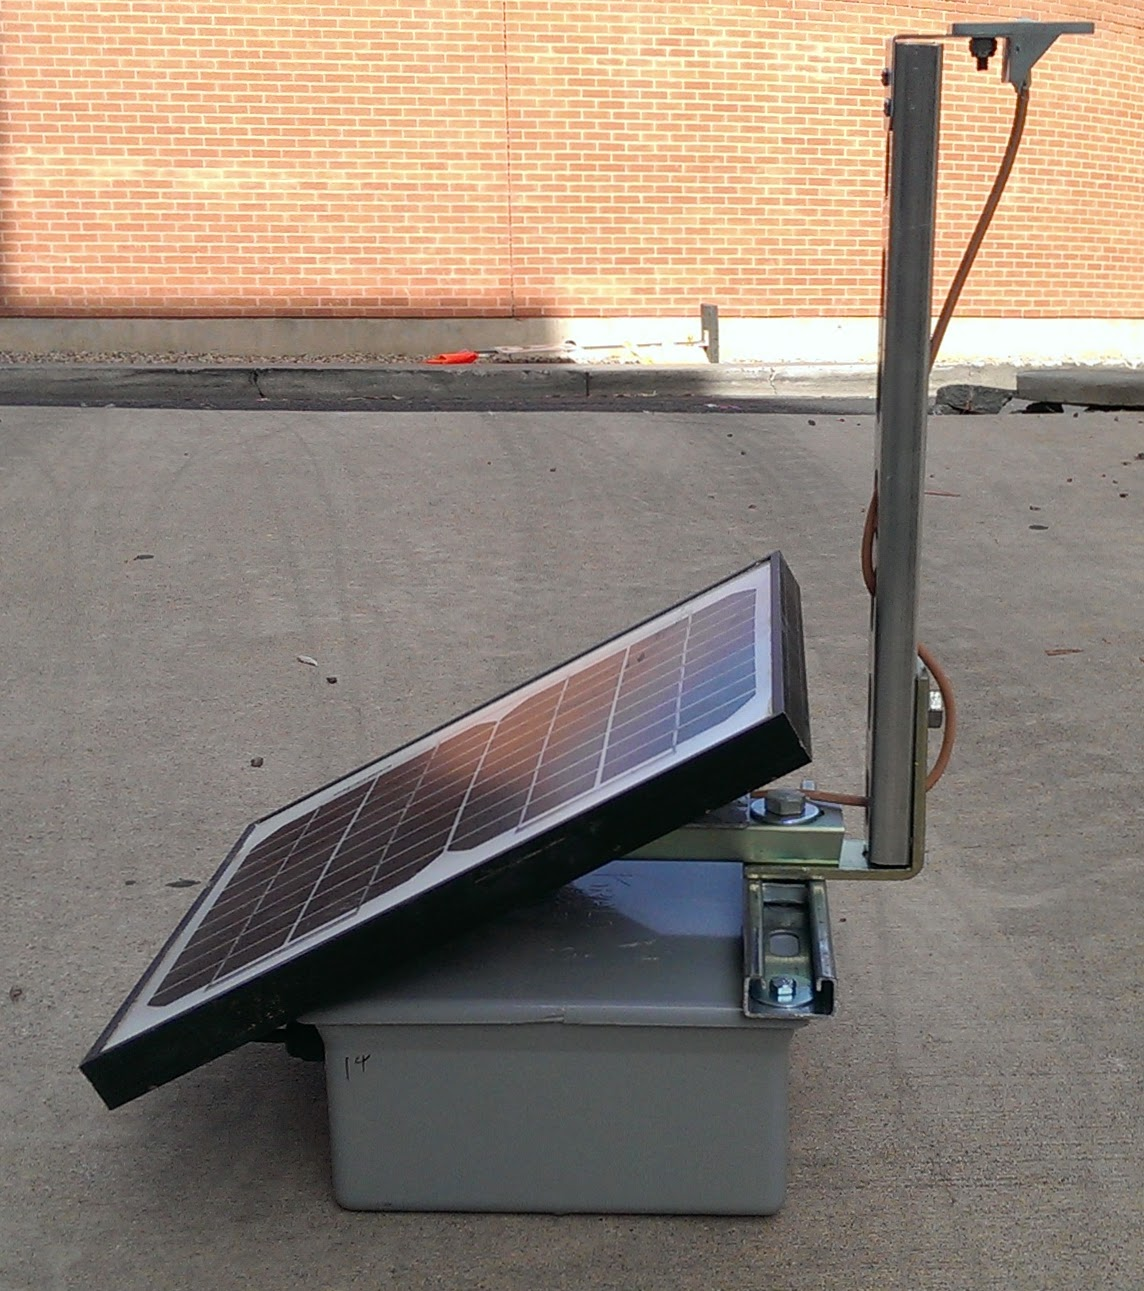
\includegraphics[width=\textwidth]{figs/sensor_outside.jpg}
\caption[A complete custom sensor]{A photo of a complete custom
  irradiance sensor as it undergoes testing outside. The photodiode
  sensor can be see mounted in the upper right of the image connected
  via a coax cable to the circuitry inside the box.}
\label{fig:sensor_outside}
\end{figure}

\subsection{Software}
Here we document the approach we took to collect and send data from
each sensor.
We compiled a Linux kernel with options to take advantage of
the GPIO and SPI capabilities of the OLinuXino board.
With this kernel, we chose Arch Linux as the operating system and
copied this base system onto an SD card with a unique system
identifier for each sensor.
Upon first boot, the system checks with a centralized server to
register itself.

Most scripts were written in Python which enabled fast prototyping.
The main data collection script is started on boot and monitored via
Supervisor to ensure it is restarted if it dies for some reason.
This script pulls data from the connected ADCs at a configurable rate,
timestamps it, and stores it in files.
This data is then uploaded to our central servers every minute where
it can be imported into a database.

A separate script monitors the wireless connection to ensure the
device maintains an internet connection.
In addition to regularly sending the status of the battery and the
board temperature for each sensor, each sensor also monitors a webpage
that can instruct a sensor to connect to a central server via SSH and
provide a reverse tunnel.
This reverses tunnel allows us to remotely login to each sensor without
knowledge of the sensor's IP address and avoiding firewall issues.

\subsection{Possible Improvements}
\label{sec:sensor_improvements}
A number of improvements can nbe made to the sensor design presented in
this section.
First, most sensor failures were a result of the enclosure and
mounting choice.
Since the sensors were simply placed on the ground, they could be
knocked over by animals or flooded during the monsoon season.
To mitigate issues like this, we recommend that sensors be mounted on
a stake.
While this would complicate deployment somewhat, it would likely
prevent sensor failure due to orientation issues (where the solar
panel is not in the sun to power the device) and some water damage.

In addition to a new enclosure and mounting desgin, a number of
improvments in electronics have been made since the sensors were first
developed.
With the rise of the Internet of Things, there now exist numerous
low-power computing devices that could replace the OLinuXino MICRO in
our design.
These new low-power devices now often come with an integrated lithium
battery charge controller.
Using lithium batteries instead of lead-acid will enable smaller,
lighter sensors.

Finally, improvments can be made to the connection to a wireless
network.
A number of M2M devices have been released that enable wireless
connectivity in low-power, integrated devices.
For example, MultiTech now manufactures a device that integrates a
processor running Linux with the wireless network hardware.
These devices may also include GPS receivers enabling precise location
of sensor devices and more accurate time keeping.

\section{Rooftop PV Systems as Sensors}
\label{sec:pv_sensors}
One major challenge with using rooftop PV systems as sensors is that
the data is often difficult to collect.
One solution we employed is to use the built-in capabilities of some
inverters to send data directly via FTP.
With the help of a local PV system installer, Technicians for
Sustainability, we are collecting 5 minute averaged power data from
over 70 systems in the Tucson area in near real-time.
Since many inverters connect to a home owners network, we also
explored using cheap Linux devices (Raspberry Pi) to communicate with
inverters on the network and upload the data to a central server.

The electric utilities also have access to inverter data, although it
may be delayed by days or weeks and aggregated to daily or longer values.
With an increase in the installation of smart inverters, utilities are
increasingly able to access inverter data in real-time.
With an appropriate data transfer system in place, one can acquire
the rooftop data from the utility, generate a forecast, and send the
forecast back to the utility.

Since irradiance is the primary driver of PV output power, power data
from rooftop PV systems can act as a proxy for irradiance.
When analyzing both power and irradiance data, a units conversion is
likely necessary.
In our work, we choose to convert all irradiance proxy data to
clear-sky index
\begin{equation}
\label{eq:clrind}
k_n(t) = \frac{y_n(t)}{y_n^{clr}(t)}
\end{equation}
where $y_n(t)$ is the measured time-series and $y_n^{clr}(t)$ the
expected time-series for sensor $n$ if the sky were clear.
This approach accounts for differences in systems such as orientation,
peak power, and shading.
Furthermore, it detrends the diurnal cycle in the data.
The clear-sky expectation should account for temperature and aerosol
effects on a given sensor in some way to produce an unbiased clear-sky
index.

\section{Network Deployment}
\begin{figure}[h]
\centering
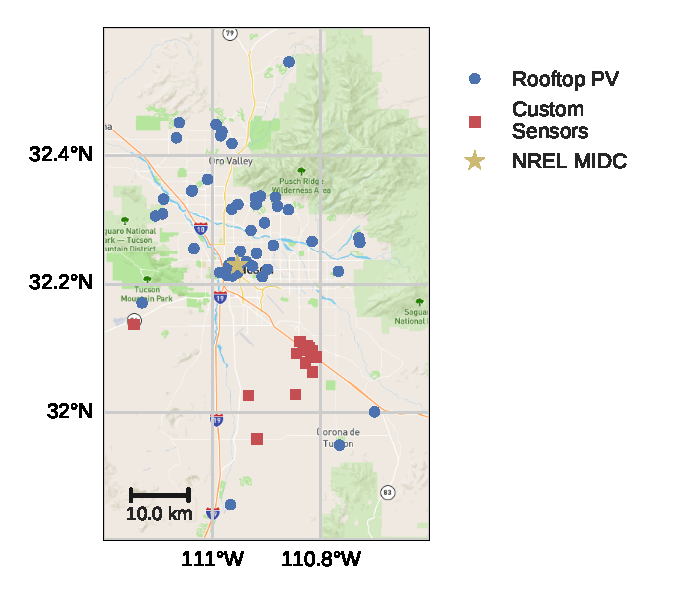
\includegraphics[width=0.75\textwidth]{figs/map.pdf}
\caption[Map of sensor locations]{Map of Tucson, AZ, indicating the
  locations of custom and rooftop PV sensors. The NREL MIDC star
  refers to the calibrated and maintened irradiance sensor located at
  the University of Arizona.}
\label{fig:map}
\end{figure}

The locations of the sensors located in the Tucson, AZ, area are shown
in \cref{fig:map}.
The blue circles denote the locations of rooftop PV systems that we
receive data from as described in \cref{sec:pv_sensors}.
The majority of these sensors are located in central and north Tucson
where the majority of homes are located.
We have no control over the placement of these sensors, but are
grateful to Technicians for Sustainability for setting up the data
transfer and to the homeowners that allow us to use the data.
The time span that data is available depends on each individual
system due to factors such as when it was installed and if the data
transfer stopped for some reason.

The red squares denote the locations of the custom sensors described
in \cref{sec:custom_sensors}.
These sensors were placed south of Tucson where there is a lack of
rooftop PV sensors.
As described in \cref{app:pvsc40}, the primary goal of this
configuration was to study forecasts for a number of PV power plants
located around $32.1^\circ$ N and $110.8^\circ$ W.
The sensors are aranged as they are based on the analysis done in
\cite{Lonij2013}, the fact that the primary cloud direction in
non-monsoon season is from the southwest, and the limited number of
sensors available.
The custom sensors shown in \cref{fig:map} were deployed in late March
2014.
Data from these sensors is available from April to July 2014, when the
sensors started failing due to monsoon rains as mentioned in
\cref{sec:sensor_improvements}.

High-quality 10 second irradiance data has been continuously gathered
from the National Renewable Energy Laboratory (NREL) MIDC OASIS sensor
hosted at the University of Arizona.
This suite of sensors (including GHI and DNI measurements) is part of
the NREL Solar Resource \& Meterological Assessment Project (SOLRMAP)
and is regularly maintained \citep{Wilcox_Andreas_2010}.
Data is publically available at \url{http://www.nrel.gov/midc/ua_oasis}.

Data from select sensors in the network supporting
\cite{Lorenzo2015c,Lorenzo2017} is available online
\citep{Lorenzo2015b,Lorenzo2016b}.
Data directly from the NREL MIDC sensor hosted at the University of
Arizona is also available \citep{Wilcox_Andreas_2010}.


%%% Local Variables:
%%% mode: latex
%%% TeX-master: "dissertation"
%%% End:

\chapter{IRRADIANCE NETWORK FORECASTS}
\label{chap:network}

Reference other sections


Background from vincent, how it's done, limitations, possible
improvements

\section{Basic Summary}
\begin{figure}[h]
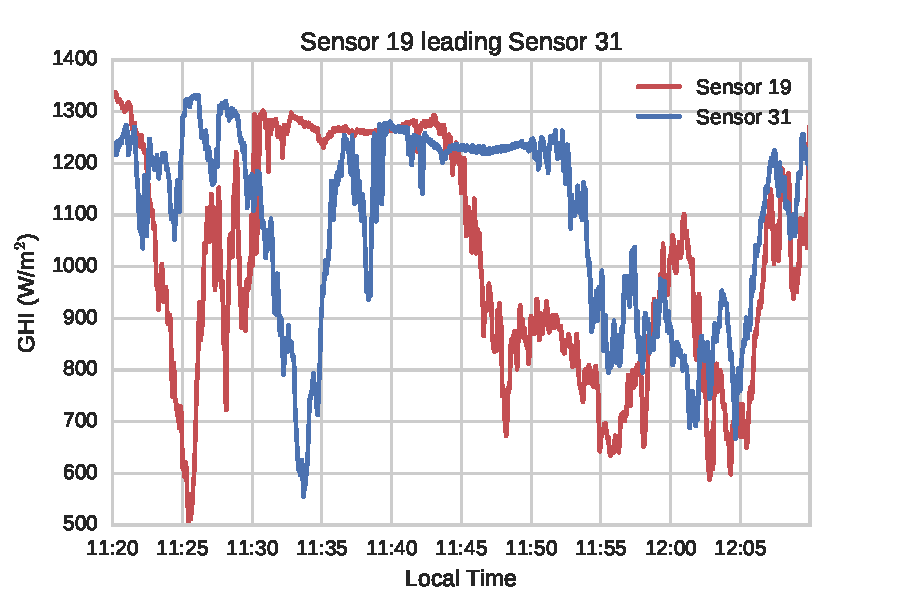
\includegraphics[width=\textwidth]{figs/leading_sens.pdf}
\caption[Example of data from one sensor predicting the output of
another]{An example of the output of sensor 19 (red) predicting what
  the output of the upstream sensor 31 (blue) in roughly 8
  minutes.}
\label{fig:leading_sens}
\end{figure}


new methods in this area

\section{Irradiance Forecast Error Metrics}
\label{sec:error_metrics}

While studying and evaluating the forecasts described in
\cref{app:network}, we learned how important it is to understand
forecast error metrics and their limitations.
Here we present an examples of possibly misleading error metrics to
warn those evaluating forecasts to be careful.

We will evaluate each metric on forecasts of clear-sky index to remove
the time of day weighting that is implicit when computing errors for
GHI.
First, we will define the error metrics to be discussed.
The most common metrics are mean bias error (MBE), mean absolute error
(MAE), and root mean squared error (RMSE) that are defined as
\begin{equation}
\mbox{MBE} = \frac{1}{N} \sum_{i=0}^N (f_i - o_i),
\end{equation}
\begin{equation}
\mbox{MAE} = \frac{1}{N} \sum_{i=0}^N |f_i - o_i|,
\end{equation}
\begin{equation}
\mbox{RMSE} = \sqrt{\frac{1}{N} \sum_{i=0}^N (f_i - o_i)^2},
\end{equation}
where $f_i$ is the forecast at time $i$ and $o_i$ is the observation
of a sensor.
MBE indicates the average bias of a forecast, and if it is not nearly
zero, bias correction techniques may be applied to the forecast to
reduce it further.
MAE indicates the average magnitude of errors as does RMSE, but RMSE
weights large errors more.

Other metrics include Pearson's correlation coefficient, the standard
deviation of the errors, and the standard deviation of the forecasts
as compared to the standard deviation of the observations.
A number of other possible useful metrics are defined
in~\cite{Zhang2015}.
We will also look at the ramp metrics defined in~\cite{Chu2015b}, the
ramp detection index (RDI), false ramp index (FRI), and ramp
magnitude forecast index (RMI).

\subsection{Example Forecasts}
Here we present forecasts for two days in Tucson, AZ, in 2014.
The first day shown in \cref{fig:5minfx_day1} has thick but broken
clouds.
The second day shown in \cref{fig:5minfx_day2} has more scattered
clouds.
In each case, observations are averaged to five minutes, Forecast A is
a five minute persistence forecast, Forecast B is a smoothing applied
to the data, and Forecast C is a fraction of the clear-sky profile for
that day.

\begin{figure}[tbp]
\centering
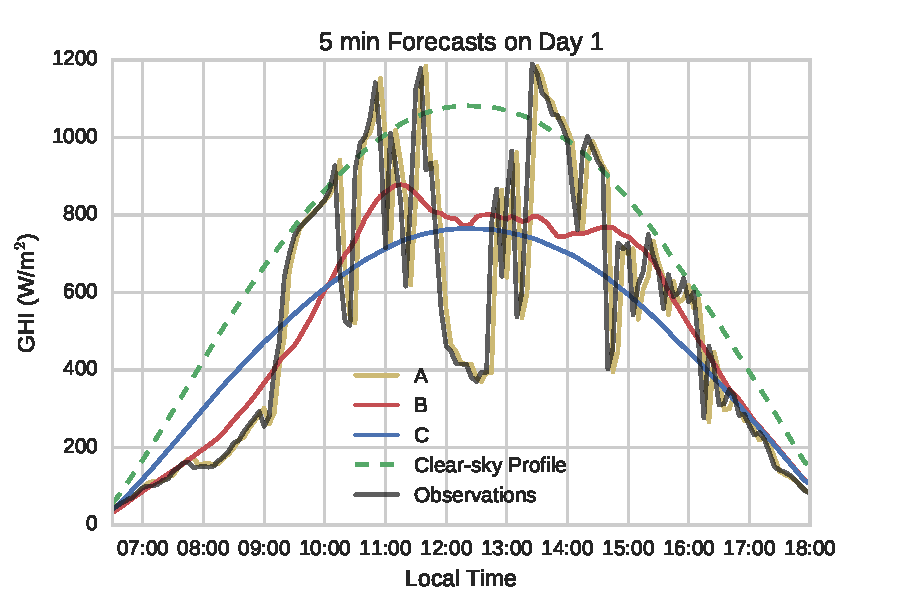
\includegraphics[width=0.8\textwidth]{figs/error_fx_Day_1.pdf}
\caption[Forecasts for a day with thick, broken clouds]{Five minute
  ahead forecasts for a day with thick broken clouds. Forecast A is a
  persistence forecast that captures the variability of the
  observations, but offset by 5 minutes. Forecast B is a somewhat
  smoothed forecast, and Forecast C is simply a fraction of the
  clear-sky profile.}
\label{fig:5minfx_day1}
\end{figure}

\begin{figure}[tbp]
\centering
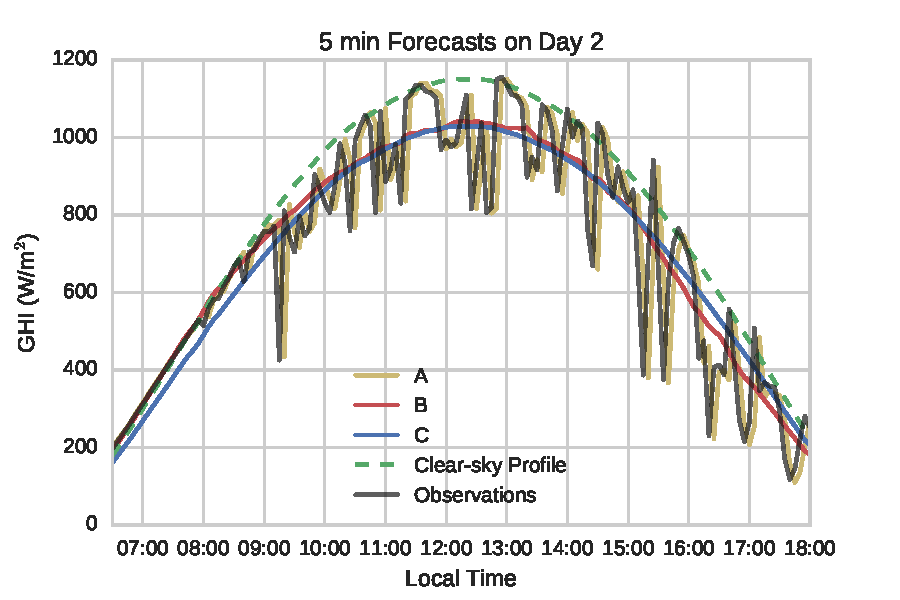
\includegraphics[width=0.8\textwidth]{figs/error_fx_Day_2.pdf}
\caption[Forecasts for a day with scattered clouds]{Five minute
  ahead forecasts for a day with scattered clouds. Forecast A is a
  persistence forecast that captures the variability of the
  observations, but offset by 5 minutes. Forecast B is a somewhat
  smoothed forecast, and Forecast C is simply a fraction of the
  clear-sky profile.}
\label{fig:5minfx_day2}
\end{figure}

Which forecast is best depends on how one plans to use the forecast.
If one is concerned with quanities like average hourly production from
a PV plant, perhaps the smoother Forecast B is best.
If one is concerned with variability to, for example, schedule
generation to back up solar power, Forecast A might be preferable.
In most cases, Forecast A is considered the better forecast that
better captures the nature of the observations.

\Cref{table:fx_errs} shows the values of some standard error metrics
for forecasts on each day.
For Day 1, Forecast A is clearly the best forecast with the lowest
MAE and RMSE, and the highest correlation to the observations.
It also performs better at detecting ramp events.
On Day 2, MAE and RMSE would suggest that Forecast B is the best.
Furthermore, Forecast C has the same RMSE as Forecast A.

\begin{table}[htbp]
\centering
\caption[Error metrics for example forecasts]{Error metrics (in units
of clear-sky index) for the forecasts on Day 1 shown in
\cref{fig:5minfx_day1} and Day 2 shown in
\cref{fig:5minfx_day2}. Refer to the text of \cref{sec:error_metrics}
for a description of each metric.}
\label{table:fx_errs}
\vspace{.3em}
\captionsetup{position=top}
\subfloat[Day 1\label{table:fx_errs_day1}]{\input{figs/Day_1_err_table}}
\hspace{3em}
\subfloat[Day 2\label{table:fx_errs_day2}]{\input{figs/Day_2_err_table}}
\end{table}

If given Forecast B or C on Day2, a user might consider it to be a
forecast of a clear day, although with possibly more aerosols in the
air reducing the irradiance slightly from the expected clear-sky
profile.
Forecast A is the only forecast to capture the variability that is
also seen in the observations and is often most concerning to
utilities.
Thus, the metrics are somewhat misleading on Day 2.

\subsection{Taylor Diagrams}
The Taylor diagram is an execellent tool to summarize a number of
metrics for many forecasts in a single figure \citep{Taylor2001}.
\Cref{fig:taylor_day1,fig:taylor_day2} are the Taylor diagrams for the
forecasts on Day 1 and Day 2, respectively.
For any forecast, the radius indicates the standard deviation of the
forecast and the angle is the correlation of the forecast with the
observations.
The gray contours indicate lines of constant centered RMSE, or RMSE
once any bias has been removed from the forecast.
A perfect forecast would lie on the x-axis (correlation = 1) and have
the same standard deviation as the observations.

\begin{figure}[p]
\centering
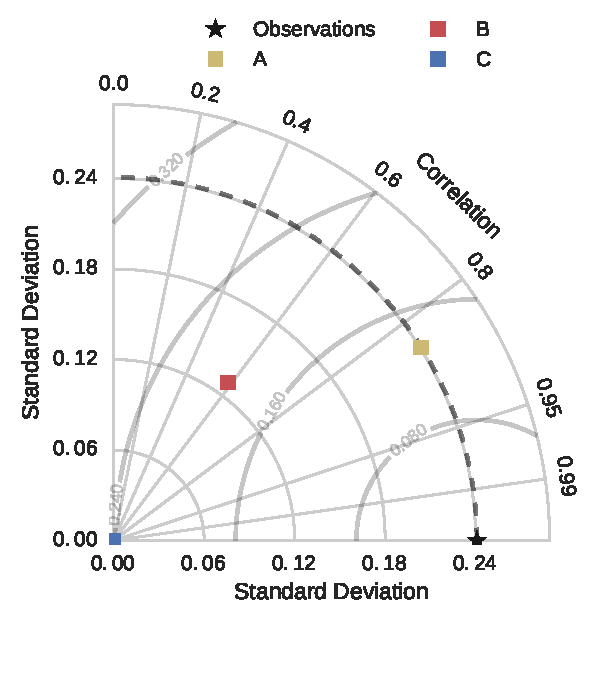
\includegraphics[width=0.8\textwidth]{figs/taylor_Day_1.pdf}
\vspace{-3em}
\caption[Taylor diagram for day 1 example forecasts]{A Taylor diagram
  for the forecasts on Day 1 shown in \cref{fig:5minfx_day1}. The
  light gray contours are lines of constant CRMSE. Forecast A has the
  lowest CRMSE in addition to having the same variability, as measured
  by the standard deviation, as the observations.}
\label{fig:taylor_day1}
\end{figure}

\begin{figure}[p]
\centering
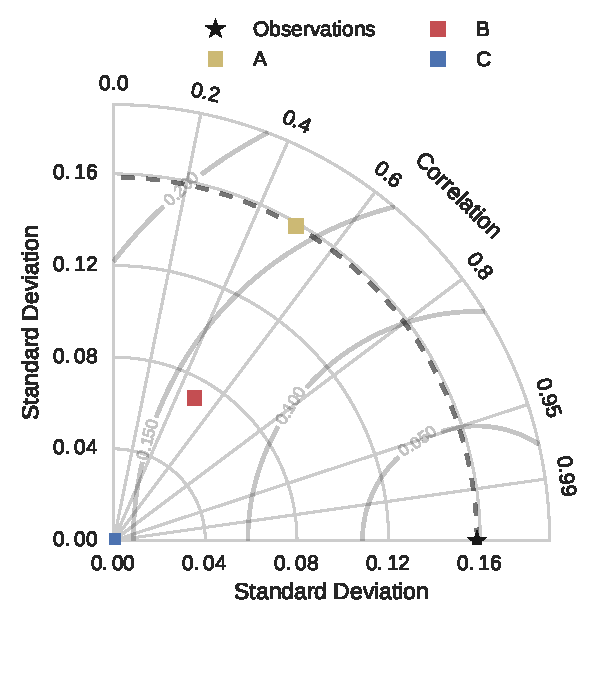
\includegraphics[width=0.8\textwidth]{figs/taylor_Day_2.pdf}
\vspace{-3em}
\caption[Taylor diagram for day 2 example forecasts]{A Taylor diagram
  for the forecasts on Day 2 shown in \cref{fig:5minfx_day2}. On this
  day, Forecast B has a smaller CRMSE and about the same correlation
  as Forecast A. However, Forecast A has similar variability to the
  observations as measured by the standard deviation. Depending on
  what the intended use of the forecast is, Forecast A may be the
  ``better'' forecast.}
\label{fig:taylor_day2}
\end{figure}

\Cref{fig:taylor_day1} confirms our assessment that Forecast A is best
on Day 1 since it has the lowest CRMSE, standard deviation equal to
that of the observations, and the highest correlation to the
observations.
From \cref{fig:taylor_day2}, Forecast A is better than Forecast C
since they have a similar CRMSE but Forecast A actually matches the
variability observed in the observations.
On the other hand, Forecast B has a lower CRMSE, but does not capture
this variability.
In this case, it depends on the use case to say whether Forecast A or
Forecast B is best.

\subsection{Suggestions}
We have hopefully demonstrated why an understanding of the error
metrics and careful application is important when evaluating
forecasts.
Evaluating forecasts on only a single or a couple of days may lead to
conflicting results, so a longer time period with varied weather
should be used when considering the overall performance of a forecast.
Furthermore, a number of metrics should be calculated and compared to
 understand the differences in forecasts, and the Taylor diagram
provides a good summary of some metrics.
Finally, an examination of the actual forecast as compared to
observations is useful to gain an intuitive sense of the forecast.

When comparing errors across studies, it is important to also consider
the region that the forecast was made for.
For example, the desert Southwest experiences fewer overcast days than
locations in the Southeast.
The Southwest also has a high number of clear days.
A forecast with low errors in the Southeast may be better at
forecasting overcast days with less skill on mostly clear days.

\section{Future Work}
velocity vectors

ensemble kalman filter

domain specific prediction

%%% Local Variables:
%%% mode: latex
%%% TeX-master: "dissertation"
%%% End:

\chapter{OPTIMAL INTERPOLATION TO IMPROVE SATELLITE NOWCASTS WITH DATA}
\label{chap:satoi}

references to other sections

- application
- basic background
- results
- extension kalman filter et

PDF and CDF?

provenance tracking?

\section{Satellite to Irradiance Algorithms}
\subsection{UASIBS}

\subsection{Empirical Model}
- based on suny

- improvments to be made

\section{Parameter Estimation}
\label{sec:paramopt}
Section 6 of \cref{app:satoi} discusses the tuning of OI for a
specific location including the estimation of the parameters
$k,\: l,\: d$ by minimizing the mean-squared error (MSE) of the
analysis over sensors withheld from OI.
To perform this minimization a grid search over the parameters was
performed and the resulting MSE for each set of parameters is shown in
\cref{fig:paramopt}.
This figure clearly shows distinct minima in parameter space for the
UASIBS satllite to irradiance model which indicates that  OI is
sensitive to the choice of parameters.
On the other hand, the lack of distinct minima in parameter space for
the empirical model indicates that a wide range of parameters would
give similar results after performing OI.
If in the future the empirical model is chosen as the background model
for an OI based routine, a more thorough investigation into why OI is
insensitive to these parameters is warranted.

\begin{figure}[p]
\centering
\captionsetup[subfigure]{labelformat=empty}
\subfloat{\hspace{-1em} 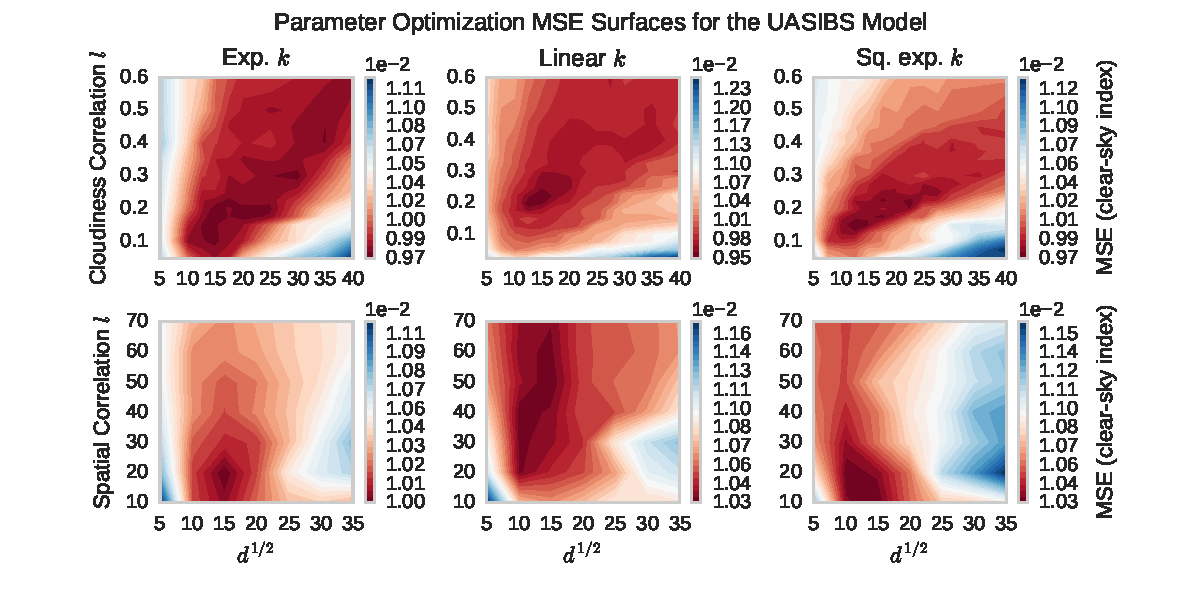
\includegraphics[width=1.05\textwidth]{figs/uasibs_optsurf.pdf}}
\vspace{-1em} \\
\subfloat{\hspace{-1em} 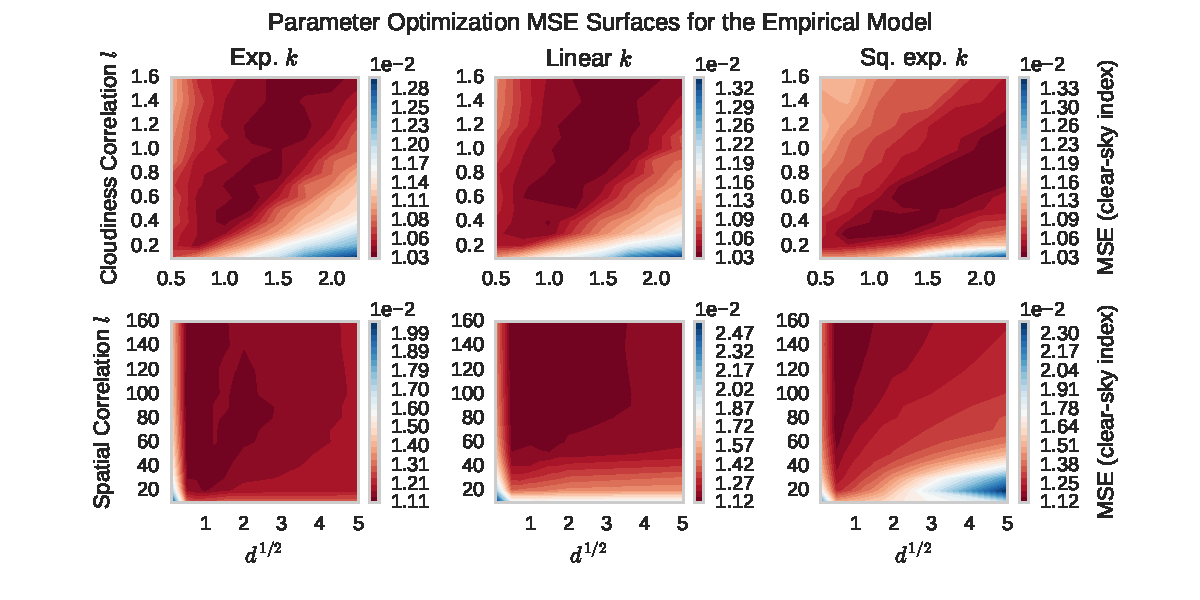
\includegraphics[width=1.05\textwidth]{figs/suny_optsurf.pdf}}
\caption[Optimization surfaces for OI parameters]{Optimization
  surfaces for the parameters $k,\: l,\: d$ of the optimal
  interpolation routine. The columns represent different choices of
  $k$, the rows distinguish between cloudiness and spatial
  correlation, the y-axis is $l$ and the x-axis is $d^{1/2}$. The top
  figure shows surfaces for the UASIBS model and the bottom is for the
  empirical model. Note, that for all choices of $k$ and the
  correlation parameterization, the surfaces for the UASIBS model have
  a clear minimum. The surfaces for the empirical model have less
  distinct minima indicating that optimal interpolation is not
  particularly sensitive to parameter choice for this model.}
\label{fig:paramopt}
\end{figure}


\section{Future Work}
(mainly pertaining to OI, mabye little bit of kalman)

new sat to irr algorithm

Here is some future work

How does NSRDB do?

GSIP?

GOES-16
%%% Local Variables:
%%% mode: latex
%%% TeX-master: "dissertation"
%%% End:

\chapter{BAYESIAN SATELLITE FORECASTS}
\label{chap:satfx}

basically way to combine chaps 2 - 4

map of all sensors (APS, TEP, rooftop, oasis, raws, isis)

ensemble forecast, multiple data sources (sensors and satellite)

multi wind ensemble

cover time horizons 1 minute to 6 hours

lots of raw compute needed

%%% Local Variables:
%%% mode: latex
%%% TeX-master: "dissertation"
%%% End:

\chapter{OPERATIONAL FORECASTING FOR UTILITIES}
\label{chap:operations}

- operational system
- large part of work
- list of scripts and what they do
- design of file interface, nabu
- speedy
- operation -> research gets used

%%% Local Variables:
%%% mode: latex
%%% TeX-master: "dissertation"
%%% End:

\chapter{CONCLUSION}
\label{chap:conc}

This dissertation has described solar irradiance forecasting
techniques that are used to produce operational solar power forecasts
for utilities.
The techniques rely on data from an irradiance sensor network.
In order to obtain such data, we designed and deployed inexpensive,
remote irradiance sensors throughout Tucson, AZ.
Using data from these sensors, we produced forecasts that improve upon
a reference by reducing RMSE by 20\% for time horizons from one minute
to two hours.
We also carefully analyzed the errors of these forecasts and described
how a smoother forecast may have smaller errors when insufficient care
is taken when analyzing errors.
For longer forecast horizons from 30 minutes to six hours, irradiance
estimates derived from satellite images are used.
Initial satellite estimates had large errors, but we used data
assimilation and data from the sensor network to cut some errors in
half.
Along the way, we studied various methods to estimate the correlation
between pixels in satellite irradiance estimates, including a novel
method based on the difference in cloudiness between two pixels.

Next steps include incorporating a cloud advection model into the data
assimilation routine to produce forecasts and to continuously
incorporate new data while retaining prior information.
These WRF forecasts used for day-ahead and longer forecasts could
benefit from incorporating the actual cloud field at the model
intialization and from an ensemble of model runs.
Eventually, a full physics large eddy simulation of the atmosphere may
be required to properly model the dynamics of clouds and to produce
good forecasts from five minutes to seven days in the future.
We will need to study how to fuse forecasting techniques together
perhaps via machine learning.


%%% Local Variables:
%%% mode: latex
%%% TeX-master: "dissertation"
%%% End:


% Include the various appendices
\appendix
\chapter{REPRINT: SHORT-TERM PV POWER FORECASTS BASED ON A REAL-TIME
  IRRADIANCE MONITORING NETWORK}
\label{app:pvsc40}
The following manuscript was published in the proceedings of the 2014
IEEE 40th Photovoltaic Specialist Conference (PVSC).
Further background material is presented in \Cref{chap:network} of
this dissertation.
The manuscript is reprinted with permission from IEEE.
Copyright (2014) by IEEE.
Original reference:
A. T. Lorenzo, W. F. Holmgren, M. Leuthold, C. K. Kim, A. D. Cronin
and E. A. Betterton, ``Short-term PV power forecasts based on a
real-time irradiance monitoring network,'' 2014 IEEE 40th Photovoltaic
Specialist Conference (PVSC), Denver, CO, 2014, pp. 0075--0079. doi:
10.1109/PVSC.2014.6925212


\newcommand{\figPV}[1]{
\begin{figure}
\includegraphics[ width=1.05\textwidth]{LorenzoPVSC40/#1}
\end{figure}
}


\figPV{pg1}
\figPV{pg2}
\figPV{pg3}
\figPV{pg4}
\figPV{pg5}


%%% Local Variables:
%%% mode: latex
%%% TeX-master: "dissertation"
%%% End:

\chapter{REPRINT: IRRADIANCE FORECASTS BASED ON AN IRRADIANCE MONITORING NETWORK, CLOUD MOTION, AND SPATIAL AVERAGING}
\label{app:network}
The following manuscript was published as a peer-reviewed article in
Solar Energy.
Further background material is presented in \Cref{chap:network} of
this dissertation.
The manuscript is reprinted with permission from Elsevier. Original
reference: A. T. Lorenzo, W. F. Holmgren, A. D. Cronin,
2015. Irradiance forecasts based on an irradiance monitoring network,
cloud motion, and spatial averaging. Sol. Energy 122, 1158--1169.
Copyright (2015) by Elsevier.

\newcommand{\figNF}[1]{
\begin{figure}
\includegraphics[ width=1.05\textwidth]{LorenzoSENF/#1}
\end{figure}
}


\figNF{pg1}
\figNF{pg2}
\figNF{pg3}
\figNF{pg4}
\figNF{pg5}
\figNF{pg6}
\figNF{pg7}
\figNF{pg8}
\figNF{pg9}
\figNF{pg10}
\figNF{pg11}
\figNF{pg12}

%%% Local Variables:
%%% mode: latex
%%% TeX-master: "dissertation"
%%% End:

\chapter{REPRINT: OPTIMAL INTERPOLATION OF SATELLITE DERIVED
  IRRADIANCE AND GROUND DATA}
\label{app:pvsc43}
The following manuscript was published in the proceedings of the 2016
IEEE 43rd Photovoltaic Specialist Conference (PVSC).
Further background material is presented in \Cref{chap:satoi} of
this dissertation.
The manuscript is reprinted with permission from IEEE.
Copyright (2016) by IEEE.
Original reference:
A. T. Lorenzo, M. Morzfeld, W. F. Holmgren and A. D. Cronin, ``Optimal
interpolation of satellite derived irradiance and ground data,'' 2016
IEEE 43rd Photovoltaic Specialists Conference (PVSC), Portland, OR,
2016, pp. 0291--0296. doi: 10.1109/PVSC.2016.7749596


\renewcommand{\figPV}[1]{
\begin{figure}
\includegraphics[ width=1.05\textwidth]{LorenzoPVSC43/#1}
\end{figure}
}


\figPV{pg1}
\figPV{pg2}
\figPV{pg3}
\figPV{pg4}
\figPV{pg5}
\figPV{pg6}


%%% Local Variables:
%%% mode: latex
%%% TeX-master: "dissertation"
%%% End:

\chapter{REPRINT: OPTIMAL INTERPOLATION OF SATELLITE AND GROUND DATA
  FOR IRRADIANCE NOWCASTING AT CITY SCALES}
\label{app:satoi}

The following manuscript was published as a peer-reviewed article in
Solar Energy.

discussed where?

The manuscript is reprinted with permission from Elsevier. Original
reference: A. T. Lorenzo, M. Morzfeld, W. F. Holmgren, A. D. Cronin,
2017. Optimal interpolation of satellite and ground data for
irradiance nowcasting at city scales. Sol. Energy 144, 466--474.
Copyright (2017) by Elsevier.

\newcommand{\figOI}[1]{
\begin{figure}
\includegraphics[ width=1.05\textwidth]{LorenzoOI/#1}
\end{figure}
}


\figOI{pg1}
\figOI{pg2}
\figOI{pg3}
\figOI{pg4}
\figOI{pg5}
\figOI{pg6}
\figOI{pg7}
\figOI{pg8}
\figOI{pg9}

%%% Local Variables:
%%% mode: latex
%%% TeX-master: "dissertation"
%%% End:

\chapter{REPRINT: AN OPERATIONAL, REAL-TIME FORECASTING SYSTEM FOR 250
  MW OF PV POWER USING NWP, SATELLITE, AND DG PRODUCTION DATA}
\label{app:wfhpvsc}
The following manuscript was published in the proceedings of the 2014
IEEE 40th Photovoltaic Specialist Conference (PVSC).
The manuscript is reprinted with permission from IEEE.
Copyright (2014) by IEEE.
Original reference: W. F. Holmgren, A. T. Lorenzo, M. Leuthold,
C. K. Kim, A. D. Cronin, and E. A. Betterton, ``An operational,
real-time forecasting system for 250 MW of PV power using NWP,
satellite, and DG production data,'' 2014 IEEE 40th Photovoltaic
Specialist Conference (PVSC), Denver, CO, 2014, pp. 0080--0084. doi:
10.1109/PVSC.2014.6925222


\newcommand{\figWPV}[1]{
\begin{figure}
\includegraphics[ width=1.05\textwidth]{HolmgrenPVSC40/#1}
\end{figure}
}


\figWPV{pg1}
\figWPV{pg2}
\figWPV{pg3}
\figWPV{pg4}
\figWPV{pg5}


%%% Local Variables:
%%% mode: latex
%%% TeX-master: "dissertation"
%%% End:


\renewcommand{\baselinestretch}{1}		% changing the value
\small\normalsize				% switch size to make the value take
\chapter{LIST OF PUBLICATIONS CO-AUTHORED BY A. T. LORENZO}
Peer-reviewed publications:
\begin{enumerate}

% e.g. \item W.F. Holmgren, R. Trubko, I. Hromada, and A.D. Cronin, \emph{``Measurement of a Wavelength of Light for Which the Energy Shift for an Atom Vanishes"} Physical Review Letters {\bf109}, 243004, (2012).
\item goes here

\end{enumerate}



\noindent Presentations and posters:

\begin{enumerate}

\item poster
%\item Low Energy Seminar, UA Physics Dept., 2010, Talk: \emph{``Absolute and ratio measurements of the polarizability of Na, K, and Rb"} W.F. Holmgren, M.C. Revelle, V.P.A. Lonij, and A.D. Cronin.

%\item Frontiers of Matterwave Optics 2010, Crete, Greece, Poster: \emph{``Absolute and ratio measurements of the polarizability of Na, K, and Rb"} W.F. Holmgren, M.C. Revelle, V.P.A. Lonij, and A.D. Cronin.

\end{enumerate}


\noindent Other works:

\begin{enumerate}

\item other stuff

\end{enumerate}

\renewcommand{\baselinestretch}{1.4}		% changing the value
\small\normalsize				% switch size to make the value take

% Switch the spacing to single-spaced for the references
\renewcommand{\baselinestretch}{1}		% changing the value
\small\normalsize				% switch size to make the value take

% Create the References list
\addcontentsline{toc}{chapter}{REFERENCES}
\bibliographystyle{ieeetran}
\bibliography{bibliography}

\renewcommand{\baselinestretch}{1.4}		% changing the value
\small\normalsize				% switch size to make the value take



\end{document}

%%% Local Variables:
%%% mode: latex
%%% TeX-master: t
%%% End:
